\chapter*{Reizen}

\begin{figure}[h]
    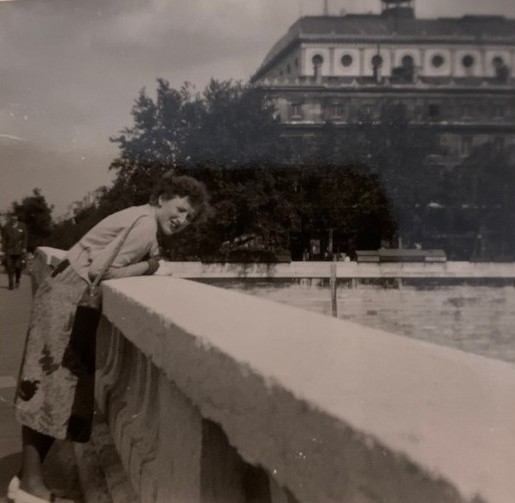
\includegraphics[width=\textwidth]{image61}
    \caption{Tiny Diks op Pont Neuf 1.}
\end{figure}

\lettrine[lines=2, loversize=0.3, lraise=0]{\initfamily I}{k} ben met Tini Diks naar Parijs geweest. Met de trein. We hebben daar van alles en nog wat bekeken. We hebben daar gelogeerd in de studentenwijk. Voor toen was dat een hele spannende reis!

En daarna ging ik natuurlijk naar London om te werken.

Ik ben ook met het vliegtuig naar Genua geweest om van daaraf met Joop mee te gaan met een kustreis. De kinderen logeerden toen bij mijn ouders. Meevaren was leuk maar ook wel saai want je had eigenlijk niet te doen. We zaten lang aan tafel!

Ik ben op mijn oude dag ook nog alleen op reis geweest naar Hongarije. Een groepsreis. Er waren best aardige mensen bij. Ik had dat wel verteld aan het begin van de reis dat ik dat niet gewend was, een groepsreis. Aan het eind vroegen ze met hoe ik het dan toch had gevonden. Ik had wel een klik met een aardige vrouw waar ik veel mee optrok. 

\begin{figure}[h]
    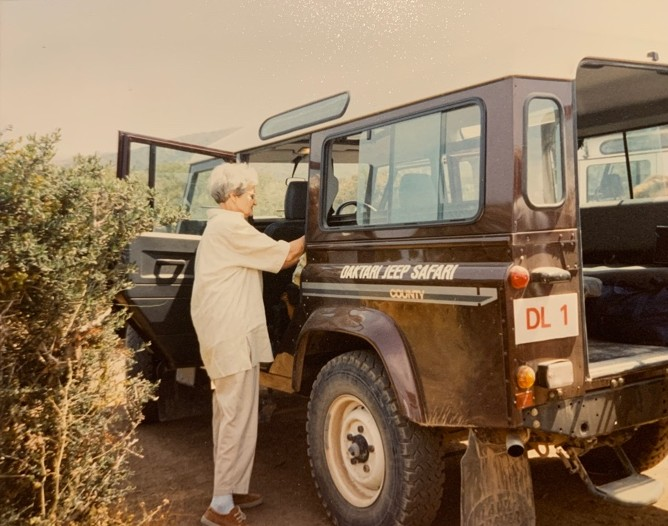
\includegraphics[width=\textwidth]{image62}
    \caption{Op reis in Cyprus.}
\end{figure}

Met mijn schoonzus Han ben ik in 1995 nog op reis geweest naar het eiland Cyprus. Dat was een erg leuke reis. Ik had een boekje dus we wisten wat we wilden zien. Een mooi eiland met grote hoogteverschillen.

\begin{figure}[h]
    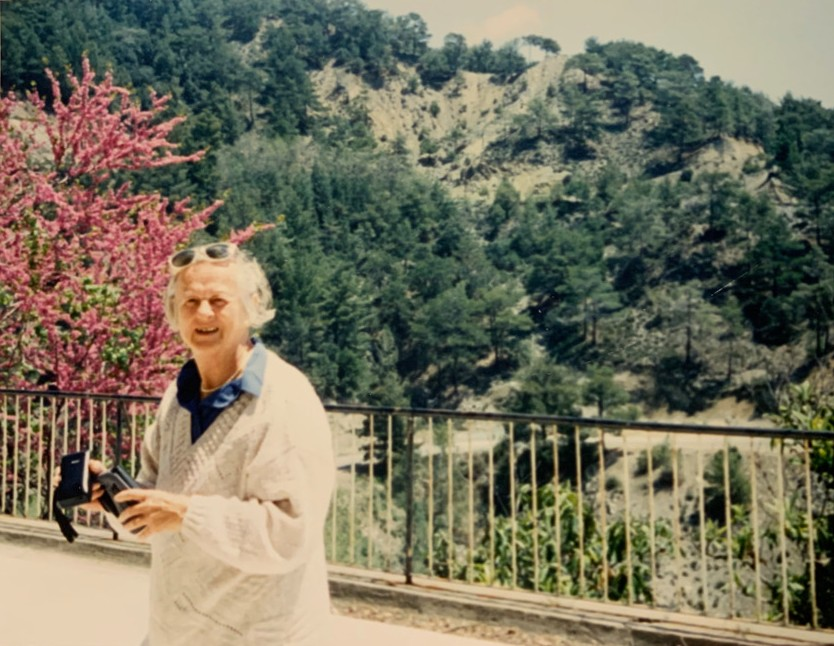
\includegraphics[width=\textwidth]{image63}
    \caption{In de natuur op Cyprus.}
\end{figure}

Han was het niet gewend dat ze zonder haar man op reis ging. Ze maakte zich zorgen of het allemaal goed zou gaan (hij dronk soms veel). Maar het was allemaal goed gegaan. Han is inmiddels al overleden. 

\begin{figure}[h]
    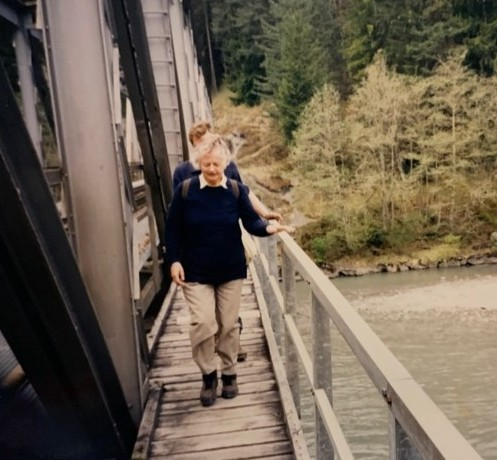
\includegraphics[width=\textwidth]{image64}
    \caption{In Zwitserland op een enge brug waar je doorheen kon kijken.}
\end{figure}
Toen ik 70 werd ben ik met de kinderen en kleinkinderen naar Zwitserland geweest. Met de bus zijn we daarheen gegaan. We hebben daar heerlijk gewandeld en ik ben met mijn hoogtevrees nog over een hele enge brug gegaan. 

\begin{figure}[h]
    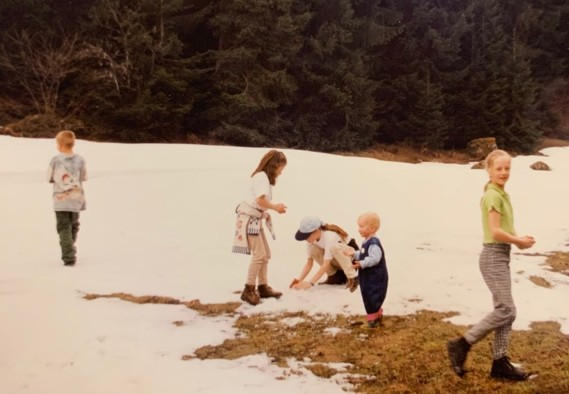
\includegraphics[width=\textwidth]{image65}
    \caption{De kleinkinderen spelen met sneeuw in Zwitserland.}
\end{figure}

\begin{figure}[h]
    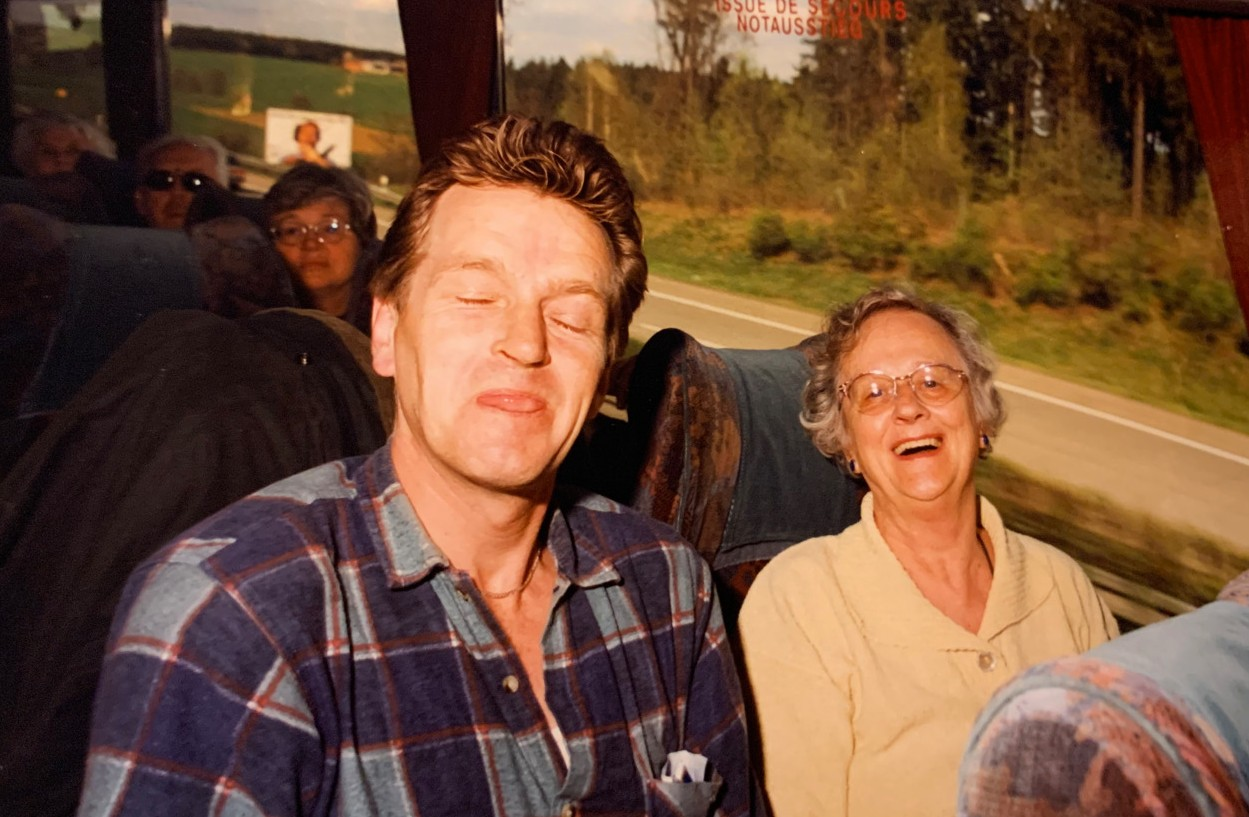
\includegraphics[width=\textwidth]{image66}
    \caption{Met Johan in de bus.}
\end{figure}


Toen Joop was overleden ging ik wel reisjes maken met de kleinkinderen. 

Met C\'{e}line en Lisa naar Wenen, samen met buurvrouw Lammie, die haar man ook had verloren. Toen waren we met de trein. 

Timon en Anne-Flore mochten mee naar Parijs, naar Disneyland. Met de trein naar Parijs en dan ging je met een speciale trein naar dat park. 

Met Anne-Flore alleen nog een keer een reisje naar Londen. 

Iliane kwam later en toen lukte het reizen niet meer zo goed. 

Met Lammie, mijn buurvrouw, ben ik nog een keer naar Valencia geweest, waar Lisa toen studeerde.

\begin{figure}[h]
    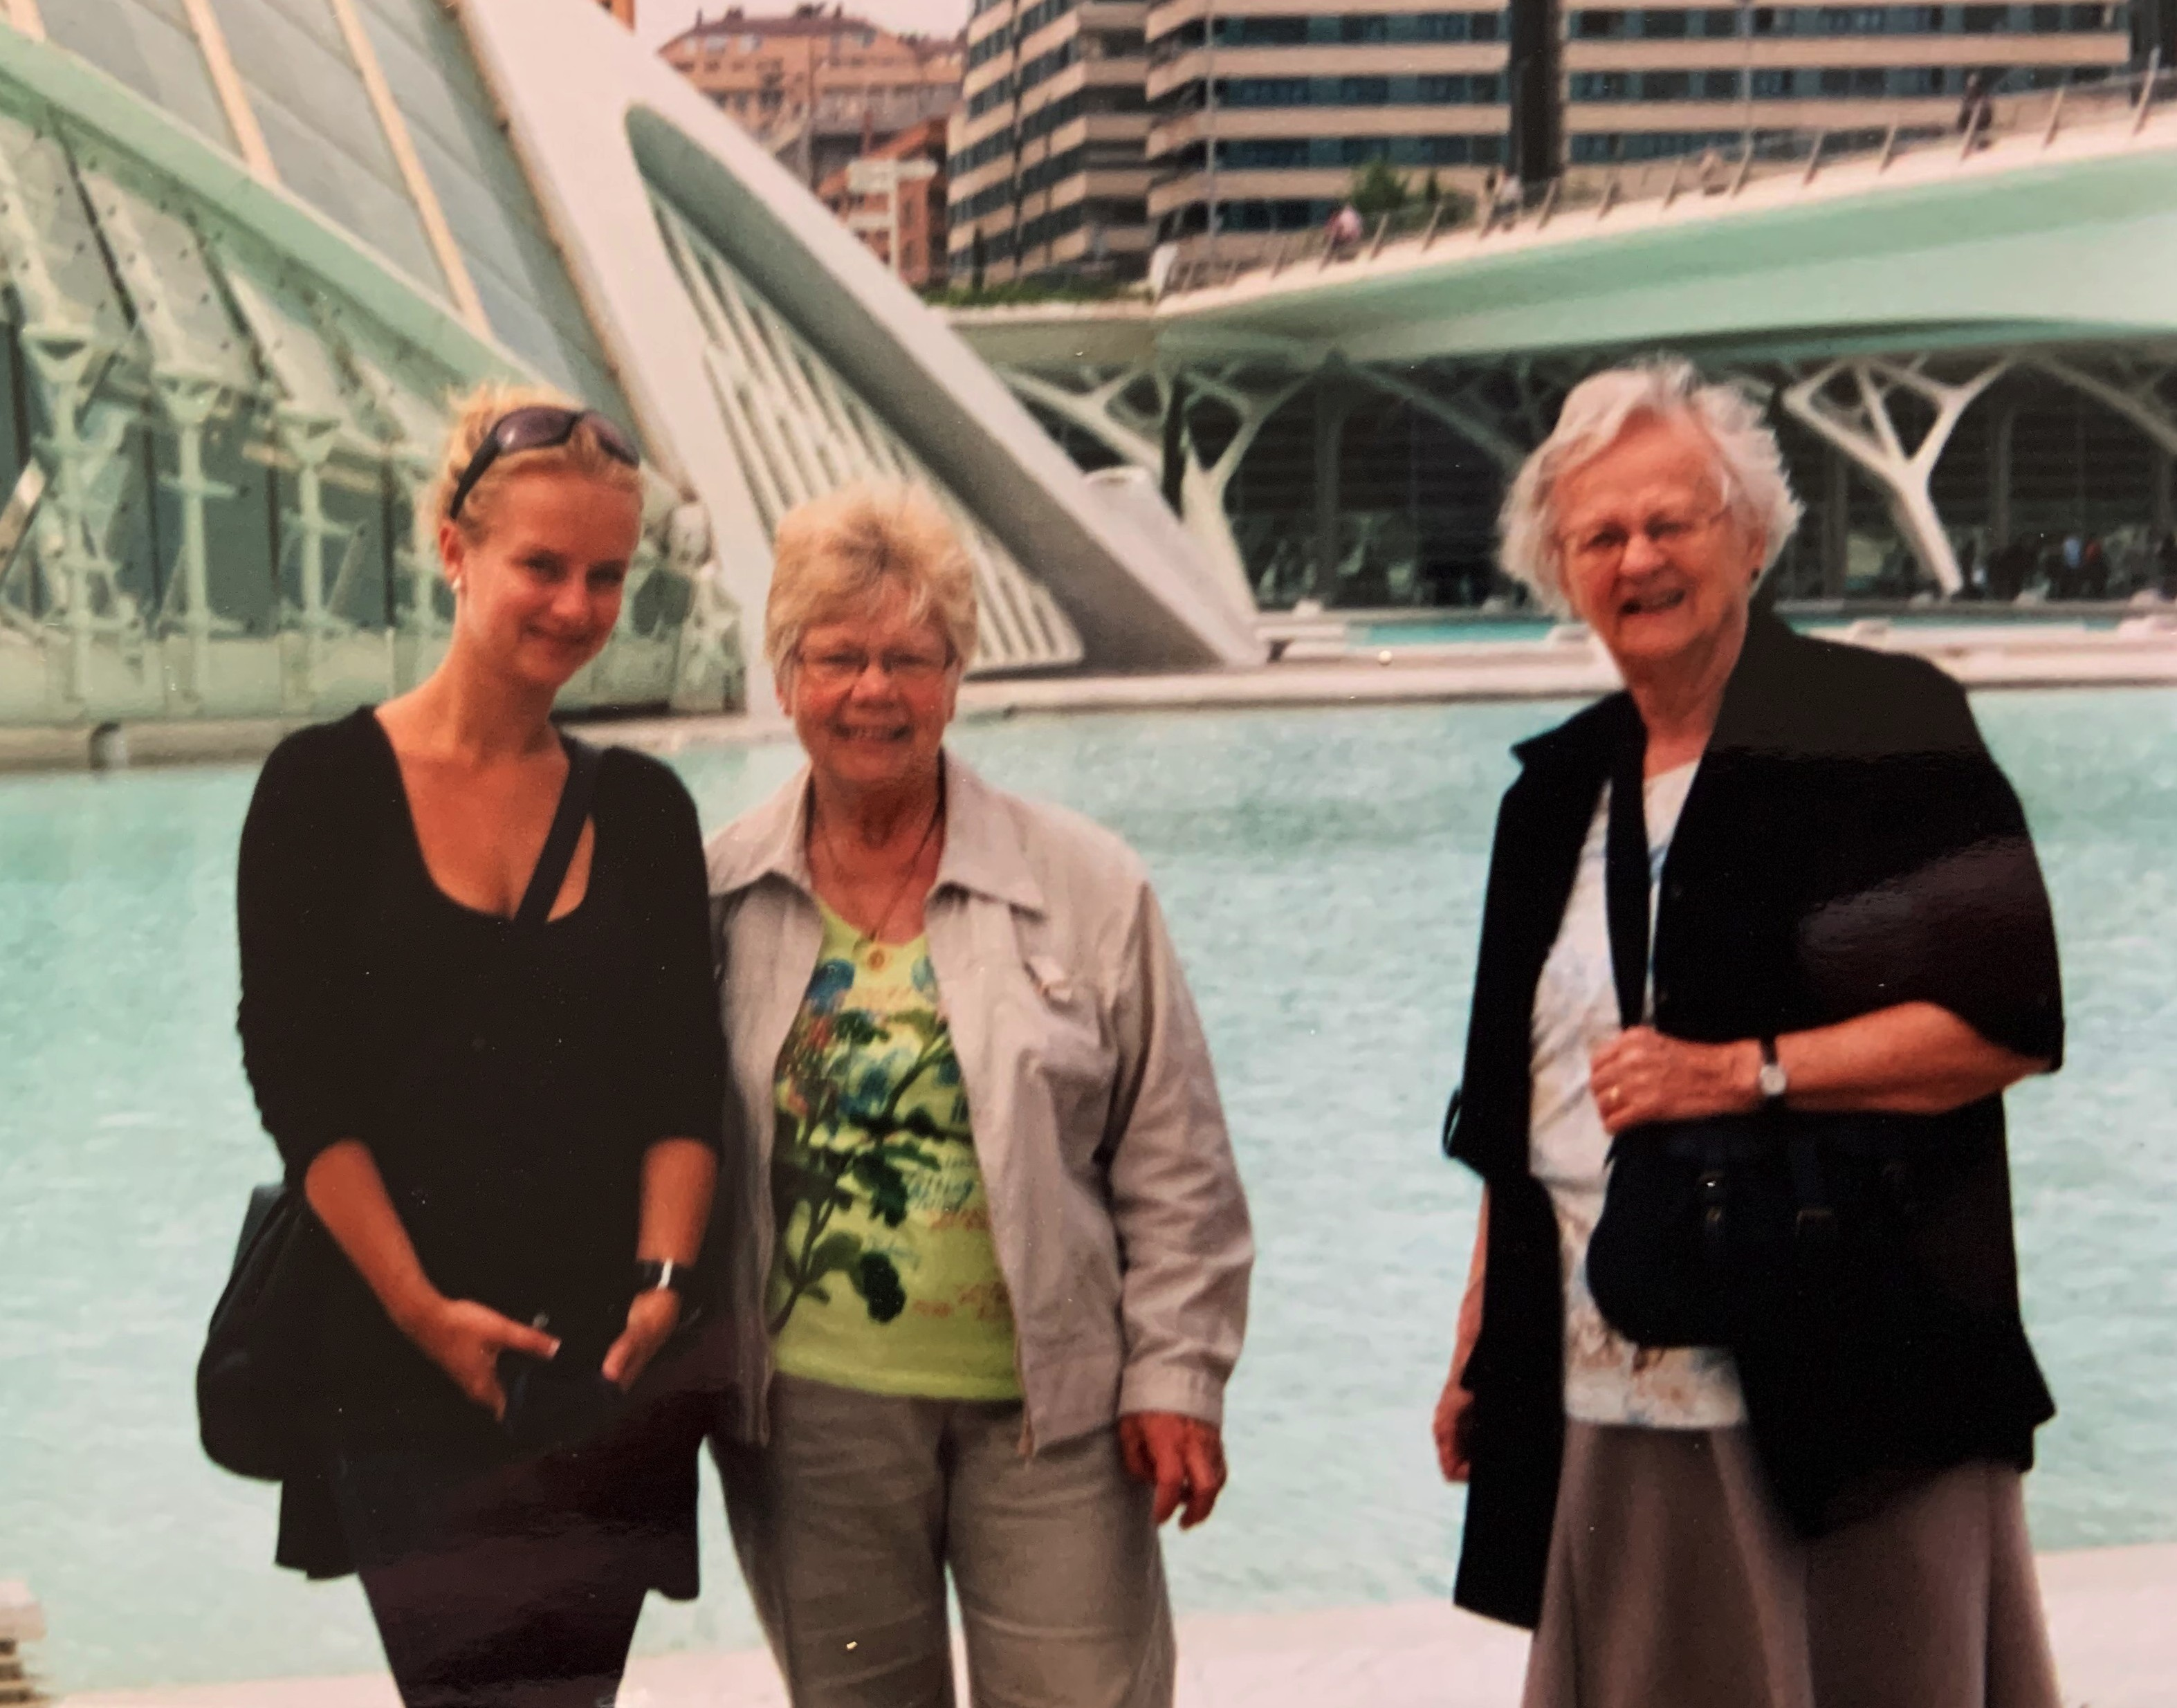
\includegraphics[width=\textwidth]{image67}
    \caption{Met Lammie op bezoek bij Lisa in Valencia.}
\end{figure}